\documentclass[master=mai,masteroption=ecs]{kulemt}
  \setup{title={Complete decision tree induction functionality in scikit-learn},
  author={Ir.\ Sven Van Hove},
  promotor={Prof.\,dr.\ Jesse Davis \and Prof.\,dr.\,ir.\ Hendrik Blockeel},
  assessor={Dr.\,ir.\ Marc Claesen},
  assistant={Elia Van Wolputte}}
  
  \setup{filingcard,
  translatedtitle=Complete beslissingsboom inductie functionaliteit in scikit-learn,
  udc=681.3*I20,
  shortabstract={500 word abstract}} %TODO copy abstract
  
  % \setup{coverpageonly}
  
  \setup{font=lm}
  
  \usepackage[pdfusetitle,colorlinks,plainpages=false]{hyperref}
  \usepackage{nameref}
  \usepackage{amsmath}
  \usepackage{amssymb}

\begin{document}

\begin{preface}
  I would like to thank Elia for the insightful discussions after business hours. I would also like to thank prof.\ Davis and prof.\ Blockeel for their helpful suggestions and the full jury for taking to time to read this document. My sincere gratitude also goes to my family and friends for their continued support. Finally, I would like to show appreciation towards my employer for the flexibility in my work schedule that made obtaining this degree possible.
\end{preface}

\tableofcontents*

\setlength{\parindent}{0cm}
\setlength{\parskip}{2ex plus 1ex minus 1ex}

% # APPROACH:
% 1. Investigate and characterize the differences in functionality between Weka and scikit-learn for decision trees.
% 2. Implement a python version of a decision tree learner that has the required basic functionality and that uses the scikit-learn interfaces.
% 3. Benchmark the developed implementation to those available in scikit-learn and Weka on a suite of datasets.
% 4. Translate the python implementation to C/cython in order to improve the run time performance.
% 5. Extend the decision tree implementation to more advance settings (e.g., online learning, …).
% 6. Provide good documentation on how the code works.

\begin{abstract} %TODO update abstract
  The \texttt{abstract} environment contains a more extensive overview of
  the work. But it should be limited to one page.~\cite{eibe2016weka}
\end{abstract}

\mainmatter%

% # BACKGROUND
% Scikit Learn (scikit-learn.org/) is well-known and increasingly popular machine learning library implemented in python. 
% Surprisingly, its implementations for some algorithm, particularly for more classical techniques such as decision trees, 
% are very incomplete with respect to the functionality provided in other packages such as Weka (http://www.cs.waikato.ac.nz/ml/weka/). 
% The missing functionality can lead to large decreases in performance. For example, we have observed that Weka can be > 25% 
% improvements in classification accuracy on some datasets compared to Scikit Learn!
% # GOAL
% Develop a (more) complete python version of decision tree learners (and possible other algorithms) that works with Scikit Learn.

\chapter{Introduction}\label{cha:intro}

% Context
% Motivation
% Goal
% Challenges

Decision tree induction is one of the most well-known tools in the machine learning community. Most of the theoretical groundwork was laid in the last three decades of the previous century. Researchers Leo Breiman and Ross Quinlan have been particularly influential in this space. Contemporary AI researchers focus most of their attentions on neural networks and in particular deep learning --- the recent hype around DeepMind's AlphaGo~\cite{alphago} victories comes to mind --- but decision tree research is not dead. Researchers still continue to propose new or improved algorithms and analyses.
%TODO mention ID3, C4.5, CART early on

Theory is one thing, but the algorithms need to be implemented as computer programs to actually be useful. Sci-kit learn~\cite{scikit-learn} is a very popular machine learning library written in Python. As such, it also contains implementations of various decision tree induction algorithms. Before sci-kit learn became popular, a Java-based library called Weka~\cite{eibe2016weka} (or ``Waikato Environment for Knowledge Analysis'' in full) was often used instead. Even today, the implementations of decision tree algorithms in Weka are still in many respects superior to those in scikit-learn. Other libraries that implement similar algorithms exist (e.g., Apache Spark~\cite{spark}), but those are beyond the scope of this text.

The goal of this thesis is to alleviate the discrepancies between sci-kit learn and Weka concerning decision tree induction. Mind that decision tree induction tools can never be truly ``complete'' as stated in the title because the field is immensely broad and still continues to grow. Nevertheless, an effort can be made to improve feature parity between these two popular tools.

\section{Thesis structure}
The structure of the remainder of this text is as follows. First, an overview of the literature study concerning decision tree induction will be presented. In particular the link between an implementation and its underlying algorithm will be clarified, including the effects of that choice on the capabilities of the tool.
%TODO structure

%motivation: problematic dataset
\chapter{Literature review}\label{cha:literature}
The relevant literature for this thesis mostly consists of papers concerning decision tree induction. These go back many decades, but fortunately there are some review and survey papers that provide a convenient overview~\cite{murthy1998automatic, rokach2005top, kotsiantis2007supervised}. On top of the academic literature, the source code and accompanying documentation of scikit-learn and Weka has also been a rich source of information.

\section{Prerequisites}
The reader ought to be familiar with basic machine learning concepts such as supervised learning, classification, regression, bias-variance trade-offs, model validation and ensemble learning. Furthermore, elementary knowledge of decision tree induction is expected. The most important basic concepts will be discussed briefly. Topics that are particularly important for the next chapters will be elaborated on.

\section{Scope}
A wide variety of decision tree induction algorithms exists. Here, only the \emph{top down induction of decision trees (TDIDT)} family is considered. It is the most common approach and it is particularly relevant to the software tools under scrutiny.

Unsupervised and semi-supervised algorithms are out of scope, as is online learning. Furthermore, only classification trees are considered. With little effort, most TDIDT classification algorithms can be converted to regression algorithms. Yet, these are far less popular and better alternatives such as XGBoost~\cite{xgboost} exist.

Ensemble methods are also out of scope. Recent decision tree algorithms rarely work with a single tree, but rather with an ensemble of trees. Random forests~\cite{rf} is a very popular example of bootstrap aggregating or \emph{bagging}. Regardless, the scope of this thesis concerns the fundamentals of decision trees, and not their derivatives. Implementation improvements suggested in this thesis could still potentially benefit related ensemble methods.

The algorithms in scope are all offline learning methods invented before the big data era. This implies that computation is done locally and that all data has to fit in memory. As such, online learning methods or distributed algorithms are out of scope.

Finally, only univariate tests are in scope. The test performed in each internal node must only evaluate one attribute of the observation. For categorical attributes, this typically implies checking whether or not the input is equal to a fixed category. For numerical (and thus ordered) attributes, the input value is compared against a fixed threshold using the less than or equal and greater than operators. Consequently, the input space is partitioned recursively using axis-aligned hyperplanes. This scope limitation precludes well-known but seldom used extensions such as oblique trees.

%TODO no rule generation
%TODO no logic trees, model trees

\section{Terminology}
Throughout the relevant literature, there is a lack of ubiquitous vocabulary shared by all researchers. Decision trees are used in various scientific fields, each with its own jargon. Specifically, there is a big divide between researchers that approach the problem from a machine learning perspective compared to those who come from a statistics background. To avoid confusion, some basic terms are reviewed. A \emph{decision tree} consists of \emph{(internal) nodes} which are connected to other nodes via a one-to-many \emph{parent-child} relation on one hand, and \emph{leaves} which have no children on the other hand. The \emph{root node} is the only node without parent. In a \emph{binary tree}, all internal nodes have two children.

Induction algorithms typically receive a \emph{training set} as input data to construct a decision tree while a \emph{test set} is used afterwards for model validation. These sets are tables of data where each row represents an \emph{observation}. All observation are fully described by a common set of \emph{attributes}. Some attributes are \emph{categorical}, others may be \emph{numeric}.\footnote{The latter is sometimes also referred to as \emph{ordered} because this is the underlying property of numbers the algorithm will use at some point. Strictly speaking categories can also have an implicit order. In that case, a good practice is to make this explicit and to convert each category to a unique number beforehand.} In a supervised learning context, one or more \emph{class labels} are also associated with each observation. If the total number of distinct class values equals two, the task is called \emph{binary classification}. Otherwise it is called \emph{multiclass classification}. \emph{Multilabel classification} occurs when one observation can be tagged with a variable number of class values at once. \emph{Multioutput classification} on the other hand occurs when multiple distinct classes, each with their own set of values, have to be derived from the same set of attributes. This can be accomplished trivially by creating multiple trees, each handling one class. Regardless, combining them in one tree might offer performance benefits. In a way, multilabel classification is a special case of multioutput classification. Decision trees are one of the few machine learning algorithms that can handle all these modes of operation natively.

During \emph{training}, first one root node is created and all observations in the training set are stored in this node. When a node is \emph{split} using some \emph{test function}, this function partitions the observations in subsets and then creates a child node for each subset. This process is repeated recursively until some stopping criterion is reached. The \emph{purity} of a node is defined as the percentage of observations in that node that belong to the majority class. A \emph{pure node} is a node with 100\% purity.

\section{A generic TDIDT algorithm}
A typical TDIDT algorithm for classification consists of two phases: a grow phase and an optional prune phase. The grow phase requires three subroutines with fixed signatures: a test generation function, a splitting function and a stopping function. Historically, researchers presented their TDIDT algorithms with fixed subroutines. Because of the common interface it is now common to choose these functions \emph{\`{a} la carte}. One could try to evaluate the performance of each function separately, but choosing the best of each function does not guarantee a global optimum. Holistic tests must be performed to ensure the best configuration is chosen. Also note that the efficacy of each combination seems to depend on the domain in which it is applied~\cite{mingers1989empirical}.

\subsection{Univariate test generation}
Based on the observations in a node, tests can be devised that spit those observations in a number of subsets. The goal of this step is to generate a finite number of tests $\tau_i \in \mathcal{T}$ based on one given attribute. Recall the tests based on multiple attributes exist but are out of scope. In the next step, one specific test is chosen from this set of possible tests.

Generating tests for categorical attributes is trivial. For binary trees the value of the attribute is compared against one specific category. If it matches, it belongs to the first subset, else to the second. This results in as many tests as there are possible categories for the attribute. For non-binary trees, one test suffices that maps each distinct category to a specific subset.

In the case of numeric, ordered attributes, threshold are introduced to partition the observations based on that ordering. That way, an infinite number of tests can be generated, which is of course undesirable. However, at least for the training data, not all tests will result in a different partitioning. A clever choice of thresholds should bring the number of subsets back to a manageable level.
%attribute selection > splitting

%ignore: categorical attributes can have an implicit ordering

\subsection{Splitting}
Classic TDIDT algorithms work by recursively splitting nodes based on some optimal test $\tau \in \mathcal{T}$, the set of all possible tests. A heuristic called the splitting criterion is required to determine this $\tau$. A few such criteria have stood the test of time.

\subsubsection{Purity}
The perfect test $\tau^*$ creates a partition $\mathcal{S}_{\tau^*} = \{S_1, \ldots, S_k\}$ wherein each subset is pure, so optimizing for weighted average partition purity is a sensible first criterion.

\begin{equation}
    p(\mathcal{S}_\tau) = \sum_i \frac{|S_i|}{|S|} p(S_i)
\end{equation}

Here, $S = S_1 \cup \ldots \cup S_k$ and $p(S)$ is the set purity as described above.
%can also be expressed as impurity instead using the same pattern as below

\subsubsection{Entropy and information gain}
In practice purity does not appear to work very well. That is why researchers came up with an alternative based on Shannon's information theory~\cite{shannon1948mathematical}. Quinlan used such metrics in many of his prominent algorithms such as ID3 and C4.5~\cite{id3ter, c45}, but it was already invented earlier for the Concept Learning System (CLS)~\cite{cls}. Define entropy (or missing information) of a variable $V$ with possible values $v_i$ and associated probabilities $p_i$ as follows:

\begin{equation}
    s(V) = - \sum_i p_i \log_2(p_i)
\end{equation}

The same concept can be applied to the class variable. Define the class entropy $s_C(S)$:

\begin{equation}
    s_C(S) = - \sum_c p(c) \log_2(p(c))
\end{equation}

where $p(c)$ is the probability that a random observation in $S$ belongs to class c. This value can be defined for any node, independent of any specific partition.

For a given test $\tau$, a similar definition can be given for each subset $S_i$ of the induced partition on $S$:

\begin{equation}
    s_C(S_i) = - \sum_c p_i(c) \log_2(p_i(c))
\end{equation}

For the entropy of the whole partition $\mathcal{S}_\tau$, again use the weighted average entropy of its subsets:

\begin{equation}
    s_C(\mathcal{S}_\tau) = \sum_i \frac{|S_i|}{|S|} s_C(S_i)
\end{equation}

Finally, calculate the information gain $h_{IG}(\tau, S)$ of the split that resulted from test $\tau$:

\begin{equation}
    h_{IG}(\tau, S) = s_C(S) - s_C(\mathcal{S}_\tau)
\end{equation}

where $\mathcal{S}_\tau$ is the partition resulting from test $\tau$.

\subsubsection{Gain ratio}
The information gain criterion is biased towards tests with many possible outcomes. This could be a problem in non-binary trees. The gain ratio alleviates this problem. First define split information $SI(\tau, S)$ --- the maximum possible information gain --- as follows:

\begin{equation}
    SI(\tau, S) = - \sum_i \frac{|S_i|}{|S|} \log_2 \frac{|S_i|}{|S|}
\end{equation}

Finally, define the gain ratio:

\begin{equation}
    h_{GR}(\tau, S) = \frac{h_{IG}(\tau, S)}{SI(\tau, S)}
\end{equation}
%watch out for instability due to very low SI! -> only calculate when high enough

In binary trees, this heuristic typically causes a less balanced tree compared to the information gain criterion~\cite{c45}.

\subsubsection{Gini}
Distance metrics such as the Gini impurity index can be used instead of heuristics based on information theory~\cite{cart}. The definitions follow the same pattern as those of the information gain:

\begin{equation}
    g(S) = \sum_c p(c)(1 - p(c))
\end{equation}
\begin{equation}
    g(S_i) = \sum_c p_i(c)(1-p_i(c))
\end{equation}
\begin{equation}
    g(\mathcal{S}_\tau) = \sum_i \frac{|S_i|}{|S|} g(S_i)
\end{equation}
\begin{equation}
    h_G(\tau, S) = g(S) - g(\mathcal{S}_\tau)
\end{equation}

% \subsubsection{Comparison}

\subsection{Stopping}
Breiman argues in his CART book~\cite{cart} that choosing good stopping criteria is far more important than choosing good splitting criteria. If early stopping was not applied or no pruning (see below) was performed afterwards, trees would grow excessively large on real world data sets. This is a classic case of overfitting. It negatively impacts many factors that make decision trees attractive in the first place, such as their comprehensibility and their fast training and inference. It is also detrimental to the performance of the model on unseen data since the model fails to generalize properly.

There are simple and more complex stopping criteria. Simples ones are based on features such as these:
\begin{enumerate}
    \item tree depth
    \item number of leaves
    \item number of observations in a node
    \item purity of a node
\end{enumerate}

More complex stopping criteria are based on the Minimum Description Length (MDL) of a tree~\cite{mdlstopping} or on statistical techniques such as a $\chi^2$-test. Quinlan proposed to use the latter in his ID3 algorithm but decided not to include it in the successor (C4.5)~\cite{id3ter, c45}.

\subsection{Pruning}
A better alternative to early stopping criteria is to let the tree grow freely, and to prune it afterwards in a bottom-up fashion. Typically, the current error estimate of the subtree rooted at the given node is compared to what the estimated error would be if this node was converted to a leaf by pruning away its descendants. If it would perform better as a leaf, the descendants are effectively pruned away. Many different pruning algorithms exists. What follows is a non-exhaustive list of common pruning approaches.

\subsubsection{Reduced Error Pruning (REP)}
Reduced Error Pruning is one of the most straightforward and statistically sound methods of pruning a tree~\cite{quinlan1987simplifying, repanalysis, elomaa2001analysis}. Instead of using the whole training set to grow the tree, some randomly chosen observations are withheld in a separate validation set. By using this validation set after the growth phase is completed, an unbiased estimate of the error of each node in the tree can be calculated. Nodes at the bottom of the tree are converted into leaves if the estimated error of the leaf is equal to or less than the estimated error of the subtree rooted at the given node. This process is repeated recursively until the smallest possible tree is obtained with the minimum estimated error based on the validation set.

The disadvantage of this method is that less data is available for growing the tree, potentially negatively impacting this process. This is not a concern if training data is available in abundance.

\subsubsection{Error Based Pruning (EBP)}
Error Based Pruning is a technique used in C4.5~\cite{c45}. It does not require a separate validation set, so the full training set can be used to grow the tree. The downside of this is that this method is less statistically sound. An upper bound is calculated based on the training error and that upper bound is used instead of the original error in comparisons. Generally speaking: if a node is associated with fewer observations, then there is less certainty about the error and the upper bound will be further away from the original value. %TODO elaborate

\subsubsection{Cost Complexity Pruning}
Cost Complexity Pruning, used in the CART algorithm~\cite{cart}, takes another approach akin to regularization in classic optimization problems. First, it generates a series of pruned trees based on the original. Then it considers both the total training error and a cost factor proportional to the size of each tree to make a first selection. If the training error increases due to the pruning, but it is compensated for by a much smaller tree, the operation as a whole can still be considered positive depending on a trade-off factor. The final tree is chosen from this first selection using a separate validation set. As such, the same drawbacks apply here as for Reduced Error Pruning.

\subsubsection{Others}
Many other pruning algorithms exist~\cite{mingers1989empirical, breslow1997simplifying, elomaa1999biases, esposito1997comparative}. The reader can find some inspiration in the following list:

\begin{enumerate}
    \item Minimum error pruning~\cite{niblett1986learning}
    \item Pessimistic pruning~\cite{mansour1997pessimistic, quinlan1987simplifying, c45}
    \item MDL-based pruning~\cite{mdlpruning, quinlan1989inferring}
    \item Critical Value Pruning~\cite{mingers1987rule}
    \item Pruning using back propagation~\cite{backproppruning}
\end{enumerate}

\subsubsection{Alternative: Rule-based Pruning}
An outlier in this list is Rule-based Pruning. Decision trees can be converted to a series of if-then statements where the condition is a conjunctive clause. These statements can be further simplified to if-then-else statements and then optimized, which can be seen as an alternative form of pruning. The resulting model is no long a tree, but it can still approximate the underlying concept that the tree used to represent.

\section{Conclusion}
TDIDT algorithms incorporate different subroutines, for each of which a number of alternatives are available. This makes them a very flexible tool with uses in a variety of settings. Popular algorithms such as C4.5 and CART are opinionated in the sense that they each propose a small number of specific configurations of components. Fortunately, that does not stop algorithm implementers from offering more choice to their users, as shown in the next chapter. Note also that there is no single precise definition of ID3, C4.5 or CART. New insights were acquired over time and added to the solution, but the algorithm name rarely changed.
\chapter{Existing implementations}\label{cha:software}
Chapter~\ref{cha:literature} discussed the theoretical basics of decision trees. In this chapter, we consider applications of this theory in the form of two popular software libraries: Weka~\cite{eibe2016weka} and scikit-learn~\cite{scikit-learn}. The focus is exclusively on Weka's J48 algorithm and scikit-learn's \texttt{DecisionTreeClassifier}. Scikit-learn only offers one other decision tree induction algorithm that performs regression instead, but that is out of scope. Weka on the other hand contains a variety of other tree builders, but most are derivatives or ensemble forms of the original J48 algorithm. Model trees and an online learner are also included, both beyond the scope of this thesis.

\section{Capabilities}
The most important difference between the two implementations regarding decision trees is in the base algorithm they started from. The J48 algorithm in Weka is based on Quinlan's C4.5~\cite{c45}, while the \texttt{DecisionTreeClassifier} in scikit-learn used CART by Breiman~\cite{cart} as the foundation. This has a profound impact on the capabilities of both implementations. These capabilities are divided in categories and discussed one by one in the following subsections.

\subsection{Structural capabilities}
CART only supports binary trees, and the same applies for scikit-learn's implementation. It is an option in J48, but the default settings generate non-binary trees. Binary trees are typically deeper than their non-binary counterparts, making the inference phase more computationally expensive. On the other hand, Elomaa et al.\ claim that the use of binary discretization with C4.5 needs about the half fitting time of using C4.5 multisplitting~\cite{elomaa1999general}. Note that this only impacts splits on categorical attributes; splits of numerical attributes are always binary.

\subsection{Input capabilities}
\subsubsection{Categorical and numerical attributes}%
\label{sssec:cat_num_attr}
ID3 was not capable of dealing with numerical attributes, but C4.5 and CART can handle both types. J48 can also handle both just like its theoretical counterpart C4.5. Scikit-learn's implementation however did not inherit the categorical input capabilities of CART. This is understandable from a software engineering perspective: scikit-learn is built on top of NumPy~\cite{numpy} which itself is a numerical, scientific computing library. The user can work around this issue by pre-processing the categorical data, using for example a \texttt{LabelEncoder}\footnote{\url{http://scikit-learn.org/stable/modules/generated/sklearn.preprocessing.LabelEncoder.html}} to map each category onto a unique ID or a \texttt{OneHotEncoder}\footnote{\url{http://scikit-learn.org/stable/modules/generated/sklearn.preprocessing.OneHotEncoder.html}} that introduces as many boolean dummy variables as there are categories where only one is active at any given category.

Consider an example where an attribute Colour contains three categories: Red, Green and Blue. By default C4.5 and Weka would generate a single test out of this attribute. Red would be mapped to the first child, Green to the second and Blue to the third (cf.~\autoref{fig:categorical_split}). CART on the other hand only generates binary trees, so it would generate three tests instead: ``Colour is Red?'', ``Colour is Green?'' and ``Colour is Blue?''. Each test has a boolean output which decides whether to jump to the left or the right child. Only two of the three tests need to be used to determine the colour: if the colour is neither Red nor Green, it is considered Blue (cf.~\autoref{fig:categorical_binsplit}). More generally, for $N$ distinct categories in an attribute, $N-1$ tests have to be performed to cover all states. Note that not all states necessarily have to be checked in a real world scenario.

In scikit-learn, a one-hot encoder is needed before the data can be processed. It would replace the Colour attribute with three numerical dummy attributes: ColourRed, ColourGreen and ColourBlue. In this case, Red is represented as $[1, 0, 0]$, Green as $[0, 1, 0]$ and Blue as $[0, 0, 1]$. Because these are numerical attributes, the test generation function will try to find thresholds to partition the space. In this case, only one threshold somewhere between 0 and 1 (e.g., 0 itself) is needed. As such, each dummy variable will cause the generation of one test: $(x \leqslant 0)$. Although the implementation is slightly different, there is a trivial isomorphism between these three tests and the three CART tests. Consequently, the semantics are preserved even though they are slightly obscured. Compare \autoref{fig:categorical_binsplit} from the previous chapter with \autoref{fig:colour_onehot} to confirm this. On a hardware level, there is no intrinsic difference in performance between the $=$ and the $\leqslant$ operator~\cite{microarchitecture}.

\begin{figure}[htp]
\begin{center}
    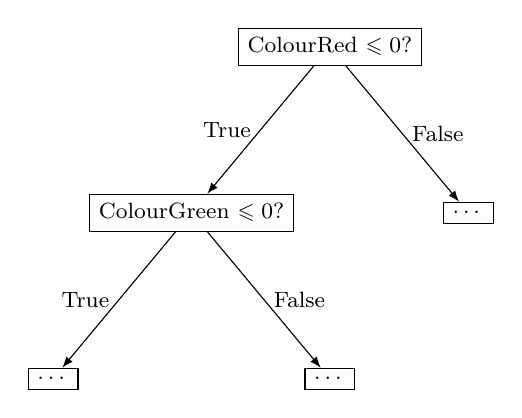
\begin{tikzpicture}
        [
            boxed/.style            = {shape=rectangle, draw, align=center},
            sibling distance        = 10em,
            level distance          = 6em,
            edge from parent/.style = {draw, -latex},
            every node/.style       = {font=\footnotesize},
        ]
        \node [boxed] {ColourRed $\leqslant 0$?}
            child { node [boxed] {ColourGreen $\leqslant 0$?}
                child { node [boxed] {\ldots} edge from parent node [left] {True} }
                child { node [boxed] {\ldots} edge from parent node [right] {False} }
                edge from parent node [left] {True} 
            }
            child { node [boxed] {\ldots} edge from parent node [right] {False} };
    \end{tikzpicture}
\end{center}
\caption{Reprise of the colour example where the data has been pre-processed using a one-hot encoding. Compared to \autoref{fig:categorical_binsplit} the structure is mirrored and the node names are less clear, but the essence remains the same.}%
\label{fig:colour_onehot}
\end{figure}

Alternatively, the label encoder would replace this categorical attribute with a single numerical attribute with possible values 0, 1 and 2. This implies that there is an order among the colours, which is not supposed to be the case. Tests such as $(x \leqslant 1.5)$ could be generated. This is equivalent to ``Colour is Red or Green?'', which is more expressive then what was possible so far. That looks positive at first, but not all logical combinations can be representation this way. In this example, no threshold can be found that implies ``Colour is Red or Blue''. Even worse, what can be represented depends entirely on the implied yet non-existent order of the original categorical variable. In short, this technique does not adhere to the original semantics and should not be used.

In conclusion, the suggested workaround with the one-hot encoder is acceptable but that does not change the fact that it negatively impact two of the decision tree advantages we listed earlier in \autoref{cha:intro}: no data preparation required and excellent comprehensibility.

\subsubsection{Missing values}
Another important input capability is dealing with missing values. As stated before, decision trees have fairly straightforward ways of dealing with this problem. While the papers on ID3 ignored this issue, both C4.5 and CART have methods for dealing with it. As before, Weka inherited the capability from C4.5, but scikit-learn did not inherit the same from CART. This is another case where extra pre-processing is needed to make decision tree induction work with scikit-learn. During this process, valuable observations might be thrown out entirely.

\subsection{Output capabilities}
\subsubsection{Classification and regression}
For this thesis regression is out of scope, but it is still an important point. CART has both classification and regression in its name, so it comes as no surprise that both are supported by this algorithm. The scikit-learn implementation is split in a \texttt{DecisionTreeClassifier} and a \texttt{DecisionTreeRegressor}. C4.5 only supports classification out of the box. Consequently, regression is not a capability of Weka's J48 implementation. However, Weka contains other decision tree algorithms, some of which do accommodate regression (e.g., \texttt{REPTree}).

\subsubsection{Multiclass, multilabel, multioutput}
On this front, scikit-learn is the superior implementation because all variants of multiclass, multilabel and multioutput are supported. Weka's J48 implementation on the other hand only supports multiclass. CART and C4.5 have the same limitations as Weka's. A simple workaround for multioutput is to fit multiple trees instead, although this might impact various performance aspects.

\subsection{Splitting criteria}
Another difference lies in the choice of splitting criteria. C4.5 and J48 support the typical criteria based on information theory such as information gain and gain ratio. CART and scikit-learn on the other hand both support information gain and the Gini impurity index but not gain ratio since it is not beneficial for binary trees. The purity criterion is not implemented in any of the algorithms due to its poor performance.

\subsection{Early stopping and pruning}
As mentioned at the end of \autoref{cha:literature}, both C4.5 and CART seemingly have their favourite pruning algorithms. The former explicitly supports Error Based Pruning and Rule-based Pruning, while the latter favours Cost Complexity Pruning. J48, like C4.5, supports Error Based Pruning by default. Quinlan's other proposal, Reduced Error Pruning, is also an option. Rule-based pruning is not supported, but Weka contains other rule based algorithms as an alternative. Of course the option not to prune at all is also available. In that case users can fall back on early stopping criteria. All algorithms and implementations include some simple stopping criteria. ID3 also introduced more complex stopping criteria, but that effort was abandoned in favour of pruning in C4.5. Breiman came to the same conclusion for CART. Surprisingly, scikit-learn did not follow Breiman's suggestion of implementing Cost Complexity Pruning. Instead, it opted for the inferior practice of using simplistic early stopping criteria such as a maximum tree depth or a minimum number of observations per node required to split it. This is by far the most significant difference between the two implementations.

\subsection{Mode of operation}
Machine learning algorithms typically operate in either one of two modes: online or offline (batch) mode. None of the algorithms and implementations under scrutiny offer online learning. Weka does include an implementation of an online tree builder (i.e., a HoeffdingTree), but not as part of J48.

\subsection{Miscellaneous}
Many more capabilities exist, but these are beyond the scope of this thesis. The interested reader can dive deeper into any of the following topics:
\begin{itemize}
    \item Generating rulesets starting for a tree representation
    \item Assigning different weights to different classes
    \item Assigning different weights to different observations
    \item Taking asymmetric misclassification costs into account
\end{itemize}

\subsection{Summary}

\begin{figure}[p]
    \centering
    \includegraphics[width=\textwidth]{img/capabilities.png}
    \caption{Summary of various capabilities as seen in the ID3, C4.5 and CART algorithms, but also in their implementations: Weka's J48 and scikit-learn's \texttt{DecisionTreeClassifier} (DTC).}%
    \label{fig:capabilities}
\end{figure}
%TODO replace with prettier visualization

Figure~\ref{fig:capabilities} shows a summary of the previous paragraphs. During the comparison of capabilities of the C4.5 and CART algorithms and their respective software counterparts Weka J48 and scikit-learn's \texttt{DecisionTreeClassifier}, three important discrepancies at the expense of the latter came up. 
\begin{itemize}
    \item It lacks pruning algorithms, making it rely on inferior simple stopping criteria instead.
    \item It cannot handle categorical attributes natively. This specifically impacts its capability of making categorical multisplits.
    \item It fails when given a training set with missing data.
\end{itemize}

Other discrepancies came up, but these were either minor or could be rationalized as explained in the previous paragraphs.

\section{Next steps}

\subsection{Lack of pruning}
The lack of pruning is a particularly noteworthy discrepancy. The current workaround involves carefully defining early stopping criteria. However, it is clearly established in the literature that this workaround is inferior to the usage of proper pruning algorithms~\cite{cart, c45}. Fixing this is priority number one. Fixing in this sense means implementing pruning algorithms for the scikit-learn decision tree induction algorithms. The next chapter immediately discusses this in more detail. In later chapters, we propose an experimental setup to evaluate the performance of the new implementation and present the results of that evaluation. Our hypothesis: pruned trees take longer to train but are smaller. That makes them less prone to overfitting so the accuracy should be the same or better and the prediction time should decrease.

\subsection{Categorical attribute handling}
Next to the lack of pruning, scikit-learn's algorithms also have a problem with categorical input. Because scikit-learn is built on top of NumPy, it uses numerical matrices to pass data between all its components. As such, categorical data simply cannot serve as input to most of its algorithms. It is part of the core philosophy of scikit-learn. Fixing this head-on would require a complete rewrite of not only the decision tree algorithms, but also all the basic interfaces and their dependencies, which is far beyond the scope of this thesis. On top of that, the use of NumPy is essential for the performance of scikit-learn. Python in itself is a slow, interpreted scripting language that is not suited for high performance computing tasks. Its integration options with C code (and the intermediate Cython code) make it a viable option, but at a considerable development cost. NumPy abstracts this complexity away behind a pure, easy to use Python interface while maintaining the speed boost.

A less significant but related discrepancy is that scikit-learn's decision tree induction implementation only generates binary trees. Breiman made this conscious choice for his CART algorithm in 1984, and it remains so today in its derivatives. Fixing this once again fundamentally changes the implementation and therefore entails a complete rewrite of the decision tree package.

In conclusion, the currently accepted workaround of pre-processing the categorical attributes in the input data using a one-hot encoder seems to be our best bet. In the upcoming chapters, we design an experiment that tests whether this workaround has any performance implications. Given the isomorphism between binary tests based on categorical attributes and binary tests based on numerical values that are the result of a one-hot encoding, we hypothesize that the performance impact is limited.

% scikit: no categorical input
%   cannot be fixed (based on numpy) without complete rewrite
% also: scikit = binary trees
%   cannot be fixed without complete rewrite (and Breiman/Weka says it's OK)
% current workaround: one-hot encoding
%   isomorphic to binary trees Weka would generate
%     except = instead of <, but performance on hardware level is same

\subsection{Missing value handling}
The third and lowest priority problem is the failure of scikit-learn to process datasets containing missing values. Three approaches are possible. The first workaround discards any observation with missing values. Depending on the context, this data loss is somewhere between irrelevant and unacceptable. The second workaround attempts to guess the values for the gaps in the data based on the rest of the data. The user must judge whether this approach is feasible in his context, but it certainly is no universal solution. For that, we look at the third option. Unlike the previous workarounds, this is not a pre-processing step. Instead, the classifier itself must be modified to deal with missing data directly. Decision tree induction algorithms typically have that capability. The C4.5 and CART texts both outline ways to deal with this problem. One option is to split an observation with a missing value into as many fake observations as there are possible values for the missing (categorical) attribute where each distinct value is used once. Some lower internal weight could be assigned to these fake observations to compensate for the data expansion.
%TODO next steps missing values?

\section{Conclusion}
This chapter introduced us to the various capabilities of decision trees. Those capabilities were mapped onto both the CART and C4.5 algorithms, but also the Weka J48 and scikit-learn implementations. This exercise revealed three important discrepancies that make scikit-learn inferior to Weka regarding decision tree induction. Those discrepancies concern pruning, categorical values and missing values. For each of these, next steps have been defined. The next chapter immediately tackles the pruning problem head-on.

\chapter{Methodology}\label{cha:method}
Intro

% Datasets + description
% Architecture?

\section{Datasets}
To evaluate the models created by the new '\texttt{PruneableDecisionTreeClassifier}, they are tested on a variety of classification datasets. These datasets are primarily taken from \url{www.openml.org}~\cite{openml}. The \emph{activity} dataset on the other hand belongs to a study by Kwapisz et al.~\cite{problematic_dataset}. In this study, the activity of a test subject is guessed based on sensor data from cell phone accelerometers. The possible activities are walking, jogging, going upstairs, going downstairs, sitting and standing. Scikit-learn's regular \texttt{DecisionTreeClassifier} performed poorly on this set in the past, although Weka's J48 handled it well. Table \ref{tbl:datasets} gives an overview.

\begin{table}
\centering
\begin{tabular}[htp]{ l l r r r l r }
    Name & Description & C & F & N & M & CF \\ \hline
    \href{https://www.openml.org/d/37}{diabetes} & Pima Indians diabetes & 2 & 8 & 768 & No & 0 \\
    \href{https://www.openml.org/d/59}{ionosphere} & Johns Hopkins ionosphere & 2 & 34 & 351 & No & 0 \\
    \href{https://www.openml.org/d/61}{iris} & Fisher's iris & 3 & 4 & 150 & No & 0 \\
    \href{https://www.openml.org/d/187}{wine} & Wine recognition & 3 & 13 & 178 & No & 0 \\
    \href{https://www.openml.org/d/1510}{wdbc} & Breast cancer Wisconsin & 2 & 30 & 569 & No & 0 \\
    \href{https://www.openml.org/d/6}{letter} & Letter image recognition & 26 & 16 & 20 000 & No & 0 \\
    \href{https://www.openml.org/d/823}{houses} & House price high/low & 2 & 8 & 20 640 & No & 0 \\
    \href{https://www.openml.org/d/53}{heart} & Heart disease & 2 & 13 & 270 & No & 0 \\
    \href{https://www.openml.org/d/334}{monks} & Monks problems & 2 & 6 & 601 & No & 6 \\
    \href{https://www.openml.org/d/50}{tic-tac-toe} & Tic-tac-toe endgame & 2 & 9 & 958 & No & 9 \\
    \href{https://www.openml.org/d/31}{credit-g} & Credit risk & 2 & 20 & 1 000 & No & 13 \\
    \href{https://www.openml.org/d/10}{lymph} & Lymphography & 4 & 18 & 148 & No & 15 \\
    \href{https://www.openml.org/d/56}{vote} & 1984 US votes & 2 & 16 & 435 & Yes & 16 \\
    \href{https://www.openml.org/d/55}{hepatitis} & Hepatitis survival & 2 & 19 & 155 & Yes & 13 \\
    % \href{https://www.openml.org/d/172}{shuttle} & Shuttle landing control & 2 & 6 & 15 & Yes & 6 \\
    \href{http://www.cis.fordham.edu/wisdm/dataset.php}{activity} & Activity prediction & 6 & 45 & 5 424 & Yes & 0 \\
\end{tabular}
\caption{Overview of classification datasets. Column C indicates the number of classes, F the number of features (excluding the class feature), N the number of observations, M whether the datasets contains missing values and CF the number of categorical features (also excluding class).}%
\label{tbl:datasets}
\end{table}

\section{Evaluation}
%grid search:
% param_grid = [
%     {
%         "prune": [None]
%     },
%     {
%         "prune": [None],
%         "min_samples_leaf": [0.5 / n_classes]
%     },
%     {
%         "prune": ['rep'],
%         "rep_test_percentage": [1/10, 1/5, 1/3, 1/2]
%     },
%     {
%         "prune": ['ebp'],
%         "ebp_confidence": [1e-5, 1e-4, 1e-3, 1e-2, 1e-1, 1/20, 1/2]
%     }
% ]
%RepeatedStratifiedKFold K=10 R=10, dataset first
%per tool per dataset, per prune method (+hyperparameters):
%n_nodes, n_leaves, accuracy, f1_weighted, fit_time, score_time (mean/std)
%random_state / seed

\section{Conclusion}

% scikit: no categorical input
%   cannot be fixed (based on numpy) without complete rewrite
% also: scikit = binary trees
%   cannot be fixed without complete rewrite (and Breiman says it's OK)
%   TODO verify in Weka whether it would make a difference
% current workaround: one-hot encoding
%   isomorphic to binary trees Weka would generate (except = instead of <)
%   both performance on hardware level is same
%   TODO verify hypothesis in Weka with and without encoding (all binary)
\chapter{Results and discussion}\label{cha:results}
In this chapter the results of the experiments detailed in the previous chapter are shown and discussed. The first section deals with pruning-related results. The next section is about categorical attributes and the final section pertains to the binary tree issue.

\section{Pruning}
In \autoref{cha:software_new}, pruning extensions were added to scikit-learn's decision tree implementations. More specifically, Reduced Error Pruning (REP) and Error Based Pruning (EBP) were implemented. In this section we evaluate how these pruning extensions affect the size of the tree (i.e., the number of nodes), the performance in terms of accuracy and the fitting and prediction speed.

\subsection{Tree size}
The mean size of the trees is shown as a heatmap in \autoref{fig:heat_nodes} for each dataset and each scikit-learn configuration. The values have been normalized by the mean size per dataset of unpruned trees. As such, the \emph{none} row which indicates that no pruning was performed is filled with 100\% values.

\begin{figure}[htp]
    \includegraphics[width=\textwidth]{img/heatmap_n_nodes.pdf}
    \caption{Mean tree size per scikit-learn configuration and per dataset. The values have been normalized by the mean size per dataset of unpruned trees. Weka results are not included in this heatmap. The colour scale goes from 0\% (white) to 100\% (black).}%
    \label{fig:heat_nodes}
\end{figure}

One value exceeds 100\%. This is possible because the pruned trees are not derivatives of the unpruned trees. They are simply two different configurations that are tested independently of each other. In this specific case, Reduced Error Pruning was used with a validation set size equal to 50\% of the training set size. Since 10\% of the dataset was already set apart in the cross-validation procedure, only 45\% of the original data was left to train the tree. Compared to the other algorithms where larger fractions of training set remain, this can profoundly change the tree structure --- including its size --- before pruning. This size is unknown, but it must have been larger than the tree size of an unpruned tree trained on 90\% of the original data. Even after pruning, the former tree turned out to be larger than the latter.

The next observation is that the other rows in the heatmap are quite light, meaning that in general the tree sizes have been reduced greatly by the various pruning strategies. For Error Based Pruning, the confidence factor plays a large role in the amount of pruning that is performed. A very low confidence factor of $10^{-5}$ results in very aggressive pruning while a factor of $10^{-1}$ results in far less pruning. The validation set size of Reduced Error Pruning on the other hand does not have a clear impact on pruning aggression. A larger validation set only results in more reliable error estimates, but on average these estimates do not move in any particular direction.

Specifically for scikit-learn, a pseudo-pruning configuration is added that uses an early stopping criterion based on the \texttt{min\_samples\_leaf} parameter instead. This is what scikit-learn users do when pruning algorithms are unavailable. As discussed earlier, it is not easy to find a good value for this hyperparameter that performs similarly across a variety of datasets. In this case the result is very aggressive pruning except for datasets wine, iris and hepatitis. This is simply because the unpruned trees of these datasets were small to begin with, and this criterion aims for a low absolute number of nodes. The other configurations also score worse on these datasets because there is less potential for pruning if there are fewer nodes to start with. \autoref{fig:unpruned_sizes} gives an overview of the mean unpruned tree size of each dataset for both scikit-learn and Weka.

\begin{figure}[htp]
    \includegraphics[width=\textwidth]{img/heatmap_n_nodes_unpruned.pdf}
    \caption{Mean size of unpruned trees (i.e., configuration \emph{none}) per dataset and per tool.}%
    \label{fig:unpruned_sizes}
\end{figure}

The first heatmap only showed results obtained from the scikit-learn configurations. The next step is to compare these results with those of Weka. \autoref{fig:heat_nodes_diff} visualizes the differences in number of nodes.

\begin{figure}[htp]
    \includegraphics[width=\textwidth]{img/heatmap_n_nodes_diff.pdf}
    \caption{Differences between scikit-learn and Weka mean tree size per configuration and per dataset. Positive numbers indicate that scikit-learn generated larger trees on average compared to Weka, and vice versa.}%
    \label{fig:heat_nodes_diff}
\end{figure}

Most of the differences are minimal. The only configuration with some larger differences is the one where pruning is not applied. The previous heatmap showed us that mean unpruned tree size can be a multiple of any mean pruned tree size. Consequently, the differences in size between unpruned trees are also larger in absolute numbers. Also note that this configuration does not involve any relevant custom code developed for this thesis. Additionally, it is proof that CART and C4.5 (and their respective implementations) do not produce the exact same trees, even when configured very similarly.

Column-wise, the letter, activity datasets --- and to a lesser extent also houses and german\_credit datasets --- stand out. These are the datasets which on average generate the largest unpruned trees, as seen in \autoref{fig:unpruned_sizes}. Percentage-wise the effect pruning has on these four datasets is in line with the other datasets. As a result, their pruned trees are on average also large. This explains the larger absolute differences. When expressed relatively in percentages, the heatmap does not show any remarkable discrepancy between these four datasets and the rest.

In conclusion, the new pruning algorithms for scikit-learn decision trees behave as expected on the structure of the trees. The resulting sizes are grosso modo the same as when the experiments are performed in Weka. The next question is whether the performance also stays the same.

\subsection{Accuracy}
\autoref{fig:heat_acc} shows a heatmap of the mean accuracy per scikit-learn configuration and per dataset. The most important observation here is that all configurations except for early stopping behave very similarly, despite large differences in the amount of pruning. Of course this is the purpose of pruning: reduce model complexity without affecting performance too much. This goal is clearly accomplished. At the same time, a strong contrast with the performance of the early stopping criterion is revealed. Across the board, it performs worse than all real pruning configurations. In the previous section we learned that early stopping acts on the tree structure the same way an aggressive pruning algorithm would. The main difference is that in general the pruning strategies are in a better position to decide whether a node is really useful. In the end, a tree of the same size but with a better node selection performs better than a tree that stopped growing prematurely because of some very generic criteria.

\begin{figure}[htp]
    \includegraphics[width=\textwidth]{img/heatmap_accuracy.pdf}
    \caption{Mean accuracy per scikit-learn configuration and per dataset. Weka results are not included in this heatmap. The colour scale goes from 50\% (black) to 100\% (white).}%
    \label{fig:heat_acc}
\end{figure}

This heatmap also clearly shows that accuracy is strongly dependent on the dataset. Not all datasets can be modelled equally well with trees (or with any classifier for that matter). Differences in class balance also exist between datasets. Accuracy as a metric can be biased when the classes are strongly unbalanced. Alternative metrics such as the F1-score are better suited in such scenarios. A similar heatmap as shown here was generated using this F1-score, but it is not included because the results were almost identical.

A small note about the result of the \emph{ebp\_0.00001} configuration on the monks dataset: the low value for the confidence value hyperparameter makes the pruner very aggressive. In this case so much that the pruned tree consists of only one node that predicts the majority class all the time.

\begin{figure}[htp]
    \includegraphics[width=\textwidth]{img/heatmap_accuracy_diff.pdf}
    \caption{Differences in percentage points (pp) between scikit-learn and Weka mean accuracy scores per configuration and per dataset. Positive numbers indicate that scikit-learn had a higher accuracy on average compared to Weka, and vice versa.}%
    \label{fig:heat_acc_diff}
\end{figure}

\autoref{fig:heat_acc_diff} reveals that these scikit-learn accuracy scores are almost perfectly in line with the Weka scores. The only real concern is the eight percentage points difference in favour of scikit-learn on the monks dataset using Reduced Error Pruning with a 50\% validation set size. Depending on which half of the data was withheld from training, the tree structure can vary dramatically. Consequently, the accuracy can vary a lot as well.
%TODO standard deviation similar, dig deeper?

The same figure also reveals that the accuracy scores on the activity dataset are almost identical between scikit-learn and Weka configurations. Even the unpruned configurations perform almost identical. This contradicts earlier reports that noticed a significant difference in performance between the two tools. We cannot reproduce this issue.

\subsection{Fitting and training time}
One last performance aspect of performance that we need to evaluate is the time taken (in milliseconds) to fit the tree and predict results with it. \autoref{fig:heat_fit} and \autoref{fig:heat_fit_diff} show the fitting time results in scikit-learn and the difference in fitting time between Weka and scikit-learn respectively. In both plots the datasets that require large trees once again stand out. This makes sense: building larger trees takes more time than building smaller trees. Weka performs worse in this aspect on such datasets. On other datasets the difference is negligible. Comparing the performance of a Java program to a Python program in terms of speed is like comparing apples and oranges, so we will not dive deeper into this topic.

\begin{figure}[htp]
    \includegraphics[width=\textwidth]{img/heatmap_fit_time.pdf}
    \caption{Mean fitting times in milliseconds per scikit-learn configuration and per dataset. Weka results are not included in this heatmap.}%
    \label{fig:heat_fit}
\end{figure}

\begin{figure}[htp]
    \includegraphics[width=\textwidth]{img/heatmap_fit_time_diff.pdf}
    \caption{Differences in mean fitting times in milliseconds between scikit-learn and Weka per configuration and per dataset. Positive numbers indicate that scikit-learn took longer on average compared to Weka, and vice versa.}%
    \label{fig:heat_fit_diff}
\end{figure}

The early stopping configuration performs the fastest fits, which is not surprising at all, but it comes at a cost in accuracy as we learned before. Pruning configurations should fit slower than the unpruned configuration because an extra step is added in this procedure. However, the results show that this is not always the case, especially when Reduced Error Pruning is applied. One possible explanation is that fewer observations are used during the growth phase. If the extra pruning phase is performed fast enough, the net result could still be faster compared to when no pruning was applied. The results support this hypothesis: the larger the validation set size, the lower the total fitting time. The Error Based Pruning configurations on the other hand behave as expected since they do not set data aside in a validation set. In that case, adding the pruning step increases total fit time. Note that these tendencies are only clearly visible when the total fitting time is large enough. In other cases, the results are lost in statistical noise.

Heatmaps of (differences in) mean prediction times are not included in this text because they do not add much value. The results are all in the range of 0--2ms, except for the letter database which takes 2--3ms for scikit-learn and 7--8ms for Weka. Due to the very low values, comparison across configurations is almost impossible and at the same time irrelevant.

\subsection{Summary}
This concludes the performance analysis of the new pruning algorithms. As expected, tree size plays a major role in explaining the subtle differences in the results. The heatmaps that show the difference in various performance aspects all reveal that scikit-learn performs very similarly to --- and sometimes even better than --- Weka. This means we successfully increased the feature parity between the two tools, which was one of the main goals of this thesis.

\section{Categorical attributes}
The second experiment investigates whether the proposed workaround for categorical variables causes a performance impact in terms of tree accuracy, fitting time and prediction time. The workaround consists of applying a one-hot encoding to all categorical attributes. As discussed in \autoref{ssec:cat_attr_handling}, this is required because scikit-learn does not support non-numerical data as input.

The experimental setup is different from the one in the previous section. A statistical test is used to determine whether there is a statistically significant difference between some averaged metric of two distinct populations (i.e., two classifier configurations). The experiment is performed in Weka, and only the \emph{ebp\_0.00100} configuration is considered because it performs most consistently with its scikit-learn mirror configuration. For more details, refer to \autoref{sec:meth_cat_attr}.

The built-in (corrected) paired T-tester of Weka reports no significant difference in accuracy for any dataset. The results are exactly the same for datasets on which the encoding has no effect: datasets without categorical attributes (the first eight entries in \autoref{tbl:datasets}) and datasets where all categorical attributes have exactly two distinct values (vote, hepatitis). That leaves four datasets: activity, monks-problems-2, tic-tac-toe and german\_credit. These four indeed show a measurable yet insignificant difference in accuracy.

The same test is repeated for the fitting time metric (measured in seconds). The pre-processing time is included in the fitting time. Since the pre-processing takes some time, there should be a significant difference for the six datasets with at least one categorical attribute. The results indeed show that these six datasets need a significantly longer fitting time, while the differences are insignificant for the other datasets. There is one unexpected finding: the houses dataset requires significantly less fitting time when (pointless) pre-processing with a one-hot encoder is applied. We have no explanation for this.

Finally, there is no significant difference in prediction time for any dataset.

A copy of the Weka analysis output is available in \autoref{sec:a1}.

In conclusion, the impact of this workaround is small to non-existent. Earlier we found that the differences between scikit-learn and Weka decision tree algorithms in general are limited. Consequently, we can reasonably assume that the same findings also apply to scikit-learn and that undertaking the challenging endeavour of rewriting scikit-learn to make it compatible with categorical attributes is unnecessary.

\section{Binary versus non-binary trees}
Although binary versus non-binary trees was not a big topic in this thesis, it is still interesting to know how the two strategies compare to each other. To that end, a similar test as in the previous section is setup up. The same remark as above is also valid here: there is no difference between the two approaches if there are no categorical attributes with at least three distinct values.

Of the four datasets where a performance difference is possible, binary trees score significantly better on accuracy for three of them. Only german\_credit shows no significant difference, just like the other datasets. In terms of fitting time, binary trees take significantly longer to train for activity and german\_credit. The other datasets show no significant difference. Finally, once again there is not a single significant difference in prediction time.

A copy of the Weka analysis output is available in \autoref{sec:a2}.

To summarize: if accuracy is the most important metric, these preliminary results suggest to stick with binary trees. If on the other hand fitting time is more important, non-binary trees are worth considering. However, in the cloud age, fitting time can easily be improved by scaling up the computing resources and introducing parallelism. Increasing performance on the other hand is not something that simply requires throwing more resources at the problem. Implementing non-binary trees in scikit-learn is a challenging endeavour, and based on these results we would not give it a high priority on the list of improvement requests.

\section{Conclusion}
Based on all the results in this chapter, we made the correct assumptions during the planning phase of this thesis. Pruning has proven to be very important, and the newly implemented pruning algorithms in scikit-learn are definitely a welcome improvement. On the other hand, it was smart to hold off on implementing non-binary trees or categorical attributes in scikit-learn, because they turned out not be as big of a problem as we first assumed.
\chapter{Conclusion}\label{cha:conclusion}
Intro

\section{Contributions}
\begin{itemize}
    \item overview of capabilities
    \item activity performance problem not reproduced
    \item pruning implementation (REP + EBP)
    \item CsvImporter: data pre-processor
    \item Categorical workaround performance test
\end{itemize}

\section{Retrospective}
\section{Future work}
\begin{itemize}
    \item missing values fix inside DT
    \item cover more edge cases (multioutput, ...)
\end{itemize}


\appendixpage*
\appendix
\chapter{The First Appendix}\label{app:A}
Appendices hold useful data which is not essential to understand the work
done in the master's thesis. An example is a (program) source.
An appendix can also have sections as well as figures and references. %TODO remove?

\backmatter%
\bibliographystyle{alpha}
\bibliography{references}

\end{document}